\documentclass[12pt,a4paper,oneside]{book}

% Packages
% Packages

% Language-related

\usepackage{setspace}
\usepackage[T1,T2A]{fontenc}
\usepackage[utf8]{inputenc}
\usepackage[english,bulgarian]{babel}

% Others
\usepackage{indentfirst}
\usepackage{amsmath}
\usepackage{blindtext} % Needed for creating dummy text passages
\usepackage[colorlinks=true,breaklinks,english]{hyperref}
\usepackage[hyphenbreaks]{breakurl}
\usepackage{xcolor}
\usepackage{ragged2e}
\definecolor{c1}{rgb}{0,0,0} % Blue
\definecolor{c2}{rgb}{0,0.3,0.9} % Light blue
\definecolor{c3}{rgb}{0.3,0,0.9} % Red blue
\hypersetup{
    linkcolor={c1}, % Internal links
    citecolor={c2}, % Citations
    urlcolor={c3} % External links/URLs
}

%\usepackage{cite} % Needed for cite

% Needed for cite and abbrvnat bibliography style
\usepackage[round,authoryear]{natbib}

% Needed for displaying bibliography and other in the table of contents
\usepackage[nottoc]{tocbibind}

\usepackage{graphicx} % Needed for \includegraphics
\usepackage{epstopdf}
\usepackage{longtable} % Needed for long tables over pages
\usepackage{bigstrut} % Needed for the command \bigstrut
\usepackage{enumerate} % Needed for some options in enumerate
\usepackage{todonotes} % Needed for todos
\usepackage{makeidx} % Needed for creating an index
\makeindex


% Page settings
% Page settings

% Needed for page border settings
\usepackage[top=1.8cm, bottom=1.8cm,left=2.0cm,right=2.0cm]{geometry}

% For writing with hyphenless justification (tries to)
\sloppy

\hyphenation{}
\hyphenpenalty=10000
\exhyphenpenalty=10000


% Custom commands

% This file defines some macros

% Text-bold-italic (makes the text bold and italic)
\newcommand{\tbi}[1]{\textbf{\textit{#1}}}

% Underline and italic
\newcommand{\imp}[1]{\underline{\textit{#1}}}


\begin{document}

\pagestyle{empty}
\begin{titlepage}

\center % Center everything on the page

\vspace{5mm}
\textsc{\Large Технологично училище Електронни системи към Технически
  университет - София}\\[0.5cm] % TUES ftw

\vspace{30mm}

{\Large \bfseries ДИПЛОМНА РАБОТА}\\[2cm]

\Large Тема: Мрежов анализатор с възможност за отдалечен анализ посредством
AngularJS 2 клиент

\vspace{40mm}

\begin{minipage}{0.35\textwidth}
\begin{flushright} \normalsize
Дипломант: \\[5mm]
Научен ръководител: \\[5mm]
\end{flushright}
\end{minipage}
~
\begin{minipage}{0.55\textwidth}
\begin{flushleft} \normalsize
Ивайло Арнаудов \\[5mm]
Стоил Стоилов\\[5mm]
\end{flushleft}
\end{minipage}\\[2cm]

{\normalsize София, $2017$} \\[0cm]


\vfill % Fill the rest of the page with whitespace

% List of symbols (kept just in case so far)

\newpage
\begin{flushleft}
\begin{Large}
\emph{\bf Списък на означения}\\
\end{Large}
\end{flushleft}
\begin{spacing}{1.241}
\vspace{10mm}
\begin{minipage}{0.2\textwidth}
\begin{flushleft} \normalsize
\ensuremath{\sigma_{y}(\tau)}\\
\end{flushleft}
\end{minipage}
~
\begin{minipage}{0.5\textwidth}
\begin{flushleft} \normalsize
Exponential regression function\\
\end{flushleft}
\end{minipage}\\[4cm]
\end{spacing}
\vfill

% List of abbreviations

\newpage
\begin{flushleft}
\begin{Large}
\emph{\bf Списък на съкращения}\\
\end{Large}
\end{flushleft}
\begin{spacing}{1.241}
\vspace{10mm}
\begin{minipage}{0.2\textwidth}
\begin{flushleft} \normalsize
VPN\\
\end{flushleft}
\end{minipage}
~
\begin{minipage}{0.5\textwidth}
\begin{flushleft} \normalsize
Virtual Private Network\\
\end{flushleft}
\end{minipage}\\[4cm]
\end{spacing}
\vfill

\pagestyle{plain}
%\listoftodos

\tableofcontents
\vfill
\chapter*{Увод}

\section{Компютърни мрежи}

Всеки от последните три века бива доминиран от някаква нова технология. Пример
за това е ерата на механичните системи съпътстващи Индустриалната революция през
XVIII век. За XIX век пък е характерен парния двигател. През XX век, ключовата
технология е събирането, обработката и дистрибуцията на информация. С развитието
й човечеството става свидетел на инсталацията на глобални телефонни мрежи,
изобретяването на радиото и телевизията, експоненциалния растеж на развитието на
компютърната индустрия и, разбира се, Интернет. Като резултат от огромния
технологичен прогрес в сферата на информационните технологии, през XXIв.
разликите между съхраняване, транспортиране и обработка на информация изтъняват,
а успоредно с това растат и изискванията на крайния потребител към
комуникационните услуги.

Въпреки крехката възраст на компютърната индустрия (напр. в сравнение с
автомобилната), тя прави значителен прогрес. През първите две десетилетия от
съществуването им, компютърните системи са били силно централизирани.
Университет или средно голяма фирма биха имали един или два компютъра, а
по-големите институции - по няколко. Идеята за съществуването на малки
устройства тип смартфон, които са взаимносвързани, е била по-скоро утопична.

Обединяването на компютрите и комуникациите оказва голямо влияние върху
организацията на самите компютърни системи. Старият модел при който един
компютър изпълнява заявките на цялата организация бива заменен от нов модел при
който голямо количество отделни, но взаимносвързани компютри извършват обработка
на дадена информация. Тези системи се наричат \textbf{компютърни мрежи}.
\cite{tanenbaum_computer_2011}
Неформална дефиниция за компютърна мрежа е множество от автономни компютри,
взаимносвързани (можещи да обменят информация помежду си) от една технология.

\section{Приложения на компютърните мрежи}

\subsection{Приложения на компютърните мрежи в бизнесa}

Обикновено повечето компании имат голямо количество компютри, най-често по един
за всеки служител. Изначално, те биха могли да работят в изолация един от друг,
но в даден момент идва необходимост те да бъдат свързани с цел служителите да
извършват работата си по-пълноценно чрез колаборация помежду си.

Един от основните проблеми, който решават компютърните мрежи е
\textbf{споделянето на ресурси}. Целта е информацията да бъде достъпна от всеки
в мрежата независимо от физическото му местоположение.

По-важен проблем, който решават компютърните мрежи е \textbf{споделянето на
информация}. Компаниите са фундаментално зависими от дигиталната
информация. Повечето компании имат записи за клиенти, за продукти и т.н. онлайн.

В допълнение, компютърните мрежи дават възможността да се използват вече
изградената мрежова инфраструктура за телефонни разговори благодарение на 
технологията \textbf{Internet Protocol (IP) телефония}, или още известна като
\textbf{Voice over IP (VoIP)}, предоставят механизми за по-богати
форми на виртуална комуникация -- споделяне на екрана
(\textbf{Desktop sharing}), видеоконференции, споделена обработка на документи.
Компютърните мрежи отварят вратите и за нов бизнес модел, наречен електронна
търговия (или \textbf{e-commerce}), който се развива с големи темпове и става де
факто стандард при търговията от всякакъв тип.  \cite{tanenbaum_computer_2011}

\subsection{Приложения на компютърните мрежи в дома}

В началото на компютърната индустрия причините за покупка на компютър от крайния
потребител са се свеждали до нужда от обработка на текст и игри. През XXI век,
основната причина е нуждата за достъп до
Интернет. Аналогично на компаниите, крайните потребители могат да достъпят
отдалечена информация, да комуникират посредством \textbf{социалните мрежи},
да купуват продукти и услуги чрез e-commerce системи, да използват електронно
банкиране, да споделят мултимедия и софтуер, да колаборират посредством
\textbf{wiki} сайтове (напр. Wikipedia).

Друго напоследък развиващо се приложение на мрежите е концепцията за 
\textbf{Internet of Things (IoT)}. Основната й характеристика е че електронните
устройства на крайните потребители се включват в компютърните мрежи; напр. душа
в банята, който традиционно не е компютър, би могъл да записва какво количество
вода е използвано и да праща информацията на приложение, което изчислява как
водата да бъде използвана възможно най-ефикасно.  \cite{tanenbaum_computer_2011}

\section{Изисквания към мрежов анализатор}

Споменатият етап на развитие на компютърните мрежи предразполага към
по-комплексни инструменти и процеси за мониторинг и отстраняване на проблеми в
мрежата. \textit{Мрежовия анализатор}, \textit{пакетен анализатор} или
\textbf{packet sniffer} е
инструмент, който помага на мрежовия администратор, предоставяйки услугата
\textit{aнализ на пакети} (\textbf{packet analysis}), още известнa като
\textbf{packet sniffing} или \textbf{protocol analysis}. Анализът на пакети
описва процеса на заснемане и интерпретиране на данни в реално време
(т.е в момента на преминаване през преносвателната среда). Изискванията към
един такъв анализататор е да улесни мрежовия администратор със изпълнението
на следните задачи:

\begin{itemize}
  \item
  Идентифициране и задълбочено разбиране на процесите в мрежата
\item
  Идентифициране на участниците в мрежата, потенциални причинители на атаки или
  злонамерена активност
\item
  Изследване кой или какво използва наличния капацитет на преносвателната
  среда, както и на моментите на максимално използване (load) на мрежата
\end{itemize}

Представеното в текущата дипломна работа приложение има за цел да спази тези
изисквания като, взимайки предвид вече описаното развитие на компютърните мрежи
с оглед необходимостта от колаборация и децентрализираност, предостави на
мрежовия администратор и възможност за отдалечено достъпване на мрежовия анализатор
както и споделен преглед на анализа с други администартори.
\justify
\chapter{Методи и технологии за реализиране на мрежови анализатори}

\section{Основни принципи, технологии и развойни среди за реализиране на мрежови
анализатори}

\subsection{Основни принципи}
Процеса на анализ на пакети включва кооперация между софтуера и хардуера и може
да бъде разделен в следните три стъпки:

\begin{itemize}
  \item
    \textbf{Събиране} В началната фаза на работата си, анализатора събира
    'сурови', неинтерпретирани данни в двоичен вид директно от проводника.
    Типично, това става като съответно избрания мрежови интерфейс за анализ
    бива превключен в т.нар.  \textbf{promiscuous mode}. В този режим, мрежовата карта
    може да 'слуша' за всевъзможен тип трафик по дадения мрежови сегмент, а не
    просто такъв, адресиран до станцията.
  \item
    \textbf{Конвертиране} В следващата фаза на работата си, анализатора
    конвертира събраните данни в разбираем формат за крайния потребител. Тук е
    мястото, където повечето добри анализатори спират с анализа. След тази
    стъпка, данните събрани от преносвателната среда са във вид, който може да
    бъде интерпретиран на много основно ниво; останалата по-голяма част от
    анализа се оставя на крайния потребител.
  \item
    \textbf{Анализ} В третата и финална фаза, мрежовият анализатор извършва
    реалния анализ на събраната и конвертирана информация. Анализатора взима
    събраните данни, отчита използвания мрежови протокол базирайки се на
    извлечените до момента данни и започва да анализира конкретните свойства на
    протокола.
\end{itemize}

С цел да бъде разбран процеса на работа, а и съответно модела на реализация на
мрежов анализатор, е необходимо дефиниране на основните принципи на
комуникация между компютърните системи.

\subsubsection{Протоколни архитектури}

За да се намали комплексността на решенията, повечето мрежи са организирани като
стек от \textbf{слоеве} или \textbf{нива}, всеки изграден върху слоя под него.
Броя на слоевете, имената на всеки от тях, съдържанието на всеки и функциите,
които изпълнява са различни за различните мрежи. Целта на всеки слой е да
предостави конкретни услуги на разположените по-високо от него в йерархията
слоеве като им спестява детайлите около имплементацията на тези услуги. 

Тази концепция е широко популярна в компютърните науки, още известна е като
криене на имплементационни детайли, абстрактни типове от данни, енкапсулация на
данни и обектно-ориентирано програмиране. Фундаменталната идея е че дадена част
от софтуера (или хардуера) осигурява услуга на потребителите си, но скрива от
тях детайлите на вътрешното си състояние и алгоритмите.

Когато слоят \textit{n} на една машина е във връзка със слоят \textit{n} на
друга машина, правилата и конвенциите използвани в тази връзка се наричат
\textbf{протокол на \textit{n}-ти слой}. На практика, протокол е договореност
между комуникиращите страни относно това как протичат процесите на
комуникацията между тях.  \cite{tanenbaum_computer_2011} Протоколите могат да
бъдат прости или комплексни. Някои от общите
свойства, които традиционно споделят, макар и абстрактно представени тук, са:

\begin{itemize}
  \item \textbf{Инициация на връзка} Дефинира кой инициира връзката, напр.
    клиентът или сървърът. При иницииране на връзка може да е необходима и
    допълнителна служебна информация преди да протече обмена на полезна
    информация.
  \item \textbf{Договаряне на параметрите на връзката} Дефинира процес, в който
    двете страни се разбират --- дали връзката е криптирана, как се пренасят
    ключовете за декриптиране, какъв тип е връзката (full/half duplex) и др.
  \item \textbf{Форматиране на данните} Дефинира подредбата на данните, в каква
    последователност се обработват от приемащата страна и др.
  \item \textbf{Откриване на грешки и корекция на грешки} Дефинира какво се
    случва при загуба на данни, как едната страна на връзката реагира при загуба
    на отгвор от другата и др.
  \item \textbf{Терминиране на връзка} Дефинира как дадено крайно устройство
    сигнализира на друго че връзката е приключила, каква финална информация
    трябва да бъде предадена преди успешния край на връзката и др.
\end{itemize}

Традиционно, тези протоколи не 'живеят' сами, а са основополагащи за цялостния
процес на комуникация.  Например, на \autoref{five_layer_network_fig} е
представен пет слоен модел на комуникация между двa софтуерни процеса. Реално
данни не се предават директно от слой \textit{n} на едната машина до слой
\textit{n} на другата: комуникацията е \textbf{виртуална} (означена с прекъснати
линии на \autoref{five_layer_network_fig}).
Вместо това, всеки слой предава данни и контролна информация на този под него
докато не се достигне най-ниския слой. Под първия слой е физическият, т.е
преносвателната среда през която реалната комуникация се случва. (означено с
непрекъснати линии на \autoref{five_layer_network_fig})

\begin{figure}[h!]
  \centering
  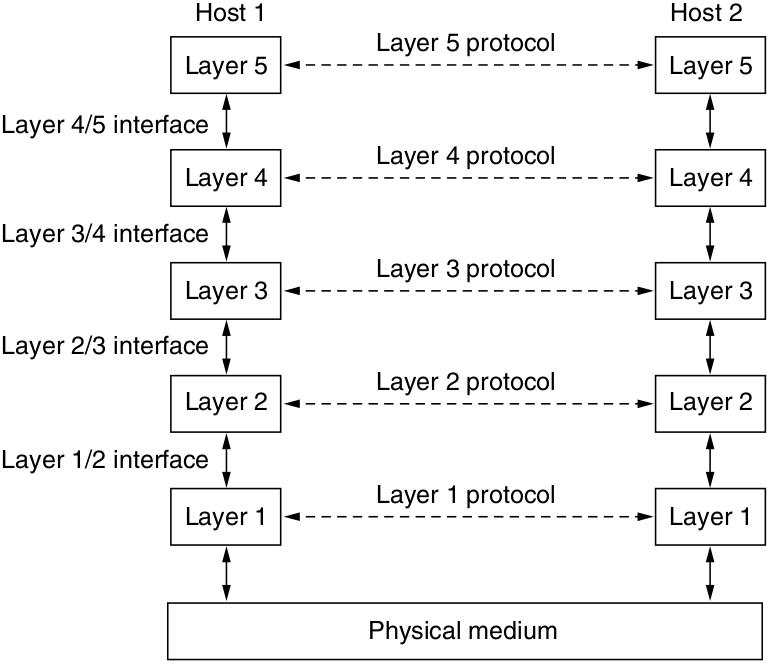
\includegraphics[width=0.7\textwidth]{figures/five_layer_network.png}
  \caption{Модел на пет слойна мрежа}
  \label{five_layer_network_fig}
\end{figure}

Между всяка съседна двойка слоеве има \textbf{интерфейс}. Този интерфейс
дефинира какви операции и услуги долният слой предлага на горния. Интерфейсите
между слоевете трябва да бъдат ясно дефинирани. Това впоследствие би улеснило
замяната на един слой с напълно различен протокол или имплементация (напр.
смяна на телефонни линии със сателитни такива), защото единственото, което се
очаква от новия протокол, е да предлага \textit{точно} същото множество услуги
на горния слой като стария. Аналогично, този механизъм позволява един протокол
да се промени в даден слой без знанието на слоевете под и над него.

\subsubsection{Основен механизъм на междуслойна комуникация. Капсулиране и
декапсулиране.}

Основния механизъм на междуслойна комуникация може да бъде описан с помощта на
пет слойния модел представен във \autoref{five_layer_network_fig}. Типично,
даден процес (т.е приложение) иска да изпрати съобщението \textit{M}. От петия
слой, съобщението бива предадено на четвъртия слой за трансмисия. Четвъртият
слой слага т.нар. \textbf{header} в началото на съобщението и предава резултата
към трети слой. Този header включва служебна информация, напр. адреси, за да
може съответния четвърти слой на приемната машина да достави съобщението. Други
примери за служебна информация могат да бъдат числови поредици (\textbf{sequence
numbers}), често използвани когато слоят на по-ниско ниво няма функционалност за
запазване на последователността на съобщенията, размери и времена.

\begin{figure}[h!]
  \centering
  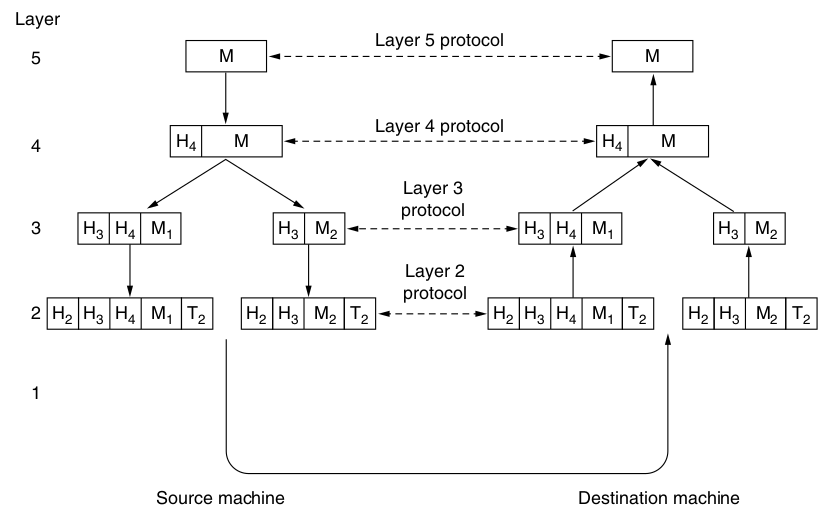
\includegraphics[width=0.8\textwidth]{figures/interlayer_communication.png}
  \caption{Междуслойна комуникация. Капсулиране и декапсулиране.}
  \label{interlayer_communication_fig}
\end{figure}

В много мрежи, често няма граница относно размера на съобщения на четвърти слой,
но почти винаги има такава относно размера от самият протокол на трети слой.
Следователно, третият слой трябва да раздели идващите съобщения на по-малки
единици --- пакети, като успоредно с това добавя header към всеки пакет. В
случая на \autoref{interlayer_communication_fig}, съобщението \textit{M} се
разделя на две части: M\textunderscript{1} и М\textunderscript{2}.

Третият слой аналогично предава пакетите на втория слой, който от своя страна
освен че добавя header, добавя и \textbf{опашка} (\textbf{trailer}). Резултата
се предава на първия слой, който се занимава с физическия пренос на данните.
Този процес е още известен като \textbf{капсулация} (\textbf{encapsulation}). В
приемащата страна, съобщението се декапсулира (\textbf{decapsulation}) като
всеки header се отделя успоредно с "изкачването" на съобщението нагоре по
слоевете. Нито един header за слоевете под \textit{n}-тия не достига до
\textit{n}-ти слой. Едновременно с това, на
\autoref{interlayer_communication_fig} ясно проличава виртуалната и реална
комуникация, както и разликите между протоколи и интерфейси. Например, на
четвърти слой процесите концептуално интерпретират комуникацията си като
хоризонтална използвайки протокола на четвърти слой и биха имали функции от типа
на send() и recieve(), въпреки че в реалност те комуникират със по-ниските
слоеве през 3/4 интерфейса, а не директно с другата страна.

\vfill

\subsubsection{Имплементации на протоколни архитектури}

\paragraph{OSI}

\paragraph{TCP/IP}

\paragraph{Основен принцип за прихваждане на данни по преносвателната среда}


Обикновенно когато мрежовата карта получи кадър (\textbf{frame}), проверява дали адресът на
получателя съвпада с нейния собствен. Ако съвпада, тя генерира прекъсване към
процесора. Функцията, обработваща прекъсването е драйвeрът за мрежовата
карта в ядрото на операционната система. Драйверът "закача" времева щампа
(\textbf{timestamp}) върху приетите данни и копира данните от буфера на картата в заделен
блок от памет в ядрото на операционната система. След това системния протоколен
стек обработва данните посредством декапсулация ги предава към
потребителското приложение.

Когато използваме мрежов анализатор, пакетите следват аналогичен път, но с малка
промяна: драйверът копира приети или изпратени данни в част от ядрото на
операционната система наречено пакетен филтър (\textbf{packet filter}) --- пакетните
филтри са в основата на функционалността на всеки анализатор. В следствие от
местоположението си, те изискват административни привилегии, тъй като
копирането на получени/изпратени пакети предполага риск за сигурността. По подразбиране,
пакетните филтри пропускат всеки пакет, но поддържат комплексни филтри. 
На \autoref{bpf_overview_fig} е илюстриран описания процес, имплементиран с
Berkley Packet Filter (BPF).

\begin{figure}[h!]
  \centering
  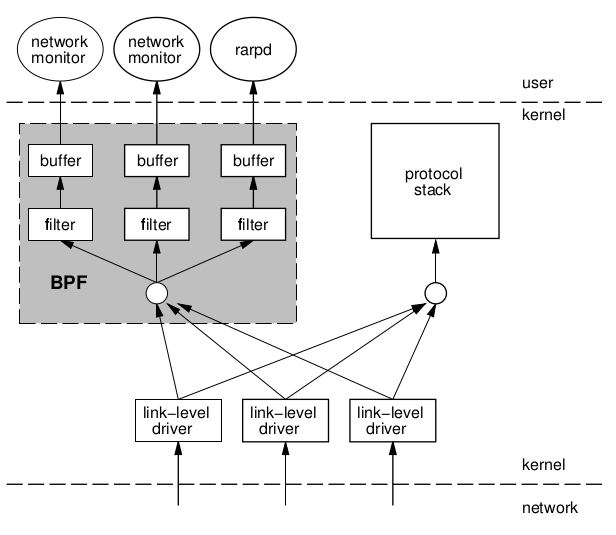
\includegraphics[width=0.7\textwidth]{figures/bpf_overview.png}
  \caption{Преглед на имплементацията на мрежов анализатор на ниво ядро на
  операционната система}
  \label{bpf_overview_fig}
\end{figure}

\subsection{Основни технологии}

\subsubsection{libpcap}

\textbf{libpcap} е библиотека с отворен код, която осигурява интерфейс на високо
ниво за системи за прихващане на пакети от преносвателната среда. Създадена е
през 1994г. от МакКейн, Лиърс и Якобсън --- изследователи в Lawrence Berkeley
National Laboratory към University of California като част от научен проект за
изследване и подобрение на TCP.  Основните цели, поставени пред библиотеката от
авторите й, са да се създаде
библиотека която е с платформенно-независим API за да се елиминира нуждата от
системно-зависими модули в приложенията на по-високо ниво, тъй като всяка
операционна система имплементира свои собствени такива механизми.

Интерфейсът на libpcap е основно достъпен на програмния език C и C\texttt{++}.
Същестуват и голямо количество библиотеки енкапсулиращи функционалността му на
езици като Perl, Python, Java, C# или Ruby. Откъм операционни системи,
libpcap се поддържа на повечето UNIX-базирани операционни систем --- 
Linux, Solaris, BSD и др. Съществува и Microsoft Windows версия, която се
нарича \textbf{winpcap}.


\subsubsection{WebSockets}

\subsubsection{AngularJS}

\subsection{Основни развойни среди}
\subsubsection{Eclipse}

The CDT Project provides a fully functional C and C++ Integrated Development
Environment based on the Eclipse platform. Features include: support for project
creation and managed build for various toolchains, standard make build, source
navigation, various source knowledge tools, such as type hierarchy, call graph,
include browser, macro definition browser, code editor with syntax highlighting,
folding and hyperlink navigation, source code refactoring and code generation,
visual debugging tools, including memory, registers, and disassembly viewers.

\subsubsection{Visual Studio}

\subsubsection{Vim}

\section{Съществуващи решения и реализации}

Преди да разгледаме същестуващите решения и реализации е важно да споменем
критериите, необходими за оценяване на полезността на един мрежов анализатор:

\begin{itemize}
  \item \textbf{Поддържани протоколи} Всички мрежови анализатори могат да
    интерпретират множество от протоколи. Повечето могат да интерпретират
    най-основните протоколи от мрежовия слой -- напр. IPv4 и ICMP; от
    транспортния слой -- TCP и UDP, както и от приложения -- DNS и HTTP.
    Не всички обаче поддържат нетрадиционни или нови протоколи (напр. IPv6).
  \item \textbf{Потребителски интерфейс} От значение е цялостния изглед на
    приложението, колко лесно се инсталира, колко лесно се извършват
    необходимите операции посредством интерфейса. От значение е и опита на
    анализиращия -- типично, по-опитният анализиращ би предпочел анализатор
    използващ командния ред, начинаещият -- анализатор с графичен интерфейс.
  \item \textbf{Цена} Голямо количество от мрежовите анализатори са
    свободно-използваеми и конкуриращи се с платени такива. Обикновенно
    разликата между платените и свободно-използваемите е при прегледа на
    анализа, който е по-пълноценнен при платените.
  \item \textbf{Програмна поддръжка} Обикновенно при изникването на проблем
    анализиращият трябва да има солидна база от източници на решения --
    документация на анализатора, публични форуми, блогове и т.н. Фундаментално
    при избора на анализатор е до колко са налични тези източници.
  \item \textbf{Поддръжка на операционната система} Не всеки анализатор поддържа
    всяка операционна система. Основополагащо за избора на анализатор е
    операционната система под която се очаква той да функционира.
\end{itemize}


\subsection{Wireshark}

Wireshark има дълга история. Програмата е оригинално създадена от Джералд Комбс,
студент по комютърни науки. Първата версия на приложението на Комбс се нарича
Ethereal и за първи път е пуснато през 1998г. под GNU Public License (GPL).  Осем
години след пускането на Ethereal, той напуска работа, но за съжаление
неговият работодател има пълни права върху името Ethereal. Така през средата на
2006г. се ражда Wireshark.

Wireshark предлага няколко предимства които я правят подходяща за всекидневна
употреба. Програмата таргетира както по-напредналите с мрежовия анализ, така и
начинаещи.

\begin{itemize}
  \item \textbf{Поддържани протоколи} Поддържа над 850 различни протокола --- от
    по-популярните като IP и DHCP, до по-комплексни частни протоколи като
    AppleTalk и BitTorrent. Вземайки предвид факта че Wireshark се разработва на
    принципа на отворения код, нов протокол се добавя с всяка нова версия. В
    случай че необходим на анализиращия протокол не е имплементиран, той може да
    бъде имплементиран като разширение и изпратен до разработчиците на
    Wireshark.
  \item \textbf{Потребителски интерфейс} Един от най-лесните за употреба
    потребителски интерфейси. Типичен Graphical User Interface (GUI) с ясно
    описани контекстни менюта и интуитивно оформление. Поддържа цветово кодиране
    спрямо протокола както и детайлен преглед на неинтерпретираните данни. За
    разлика от tcpdump, Wireshark GUI е идеална за начинаещия в мрежовия анализ.
    Разделен е на три компонента: Packet List (списък от пакети),
    Packet Details (детайли за избрания пакет), Packet Bytes (преглед на пакета
    в неинтерпретиран вид). Цялостен изглед на интерфейса може да бъде видян на
    \autoref{wireshark_fig}.
  \item \textbf{Цена} Тъй като програмата се разработва на принципа на отворения
    код, тя е изцяло безплатна и може да се използва според GPL лиценза.
  \item \textbf{Програмна поддръжка} Тъй като програмата се разработва на
    принципа на отворения код, тя няма формална поддръжка --- тя се
    базира на обществото от потребители на програмата. Уеб страницата на
    Wireshark има връзки към няколко форми за поддръжка: онлайн документация,
    wiki за разработчици, FAQ, както и връзки към официалната мейл листа.
  \item \textbf{Поддръжка на операционната система} Поддържа всички модерни
    операционни системи, вкл. Microsoft Windows, Mac OS X и Linux базираните
    операционни системи.
\end{itemize}

\begin{figure}[h!]
  \centering
  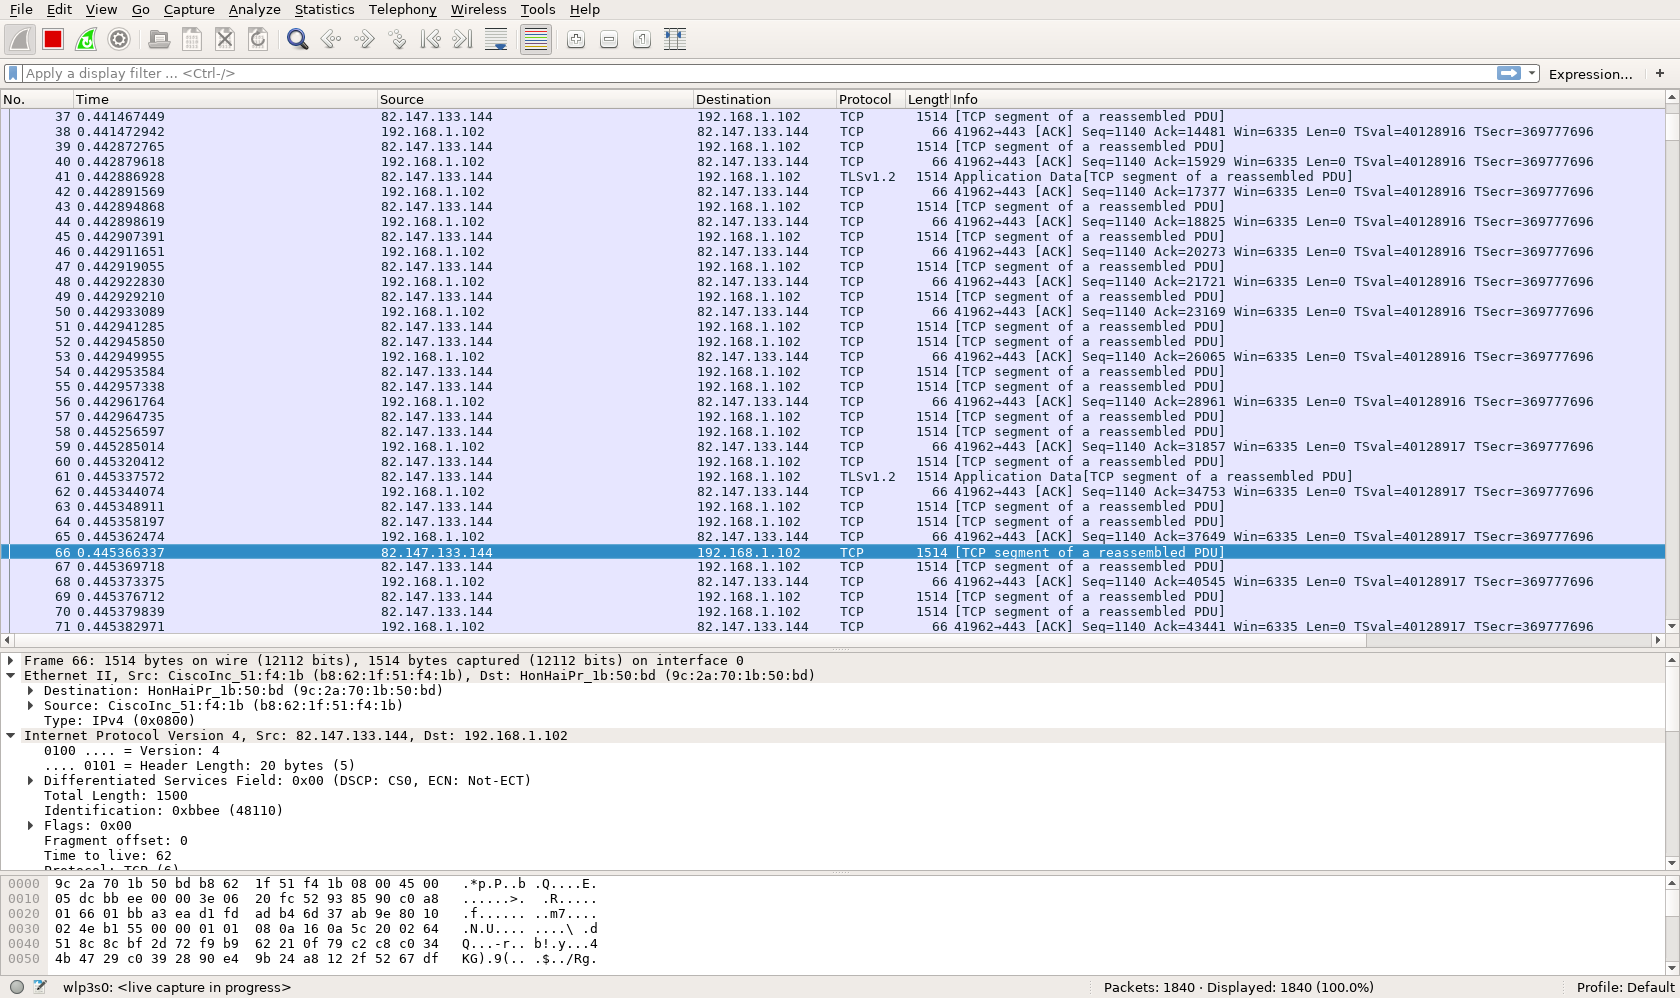
\includegraphics[width=1.0\textwidth]{figures/wireshark.png}
  \caption{Изглед на потребителския интерфейс на Wireshark.}
  \label{wireshark_fig}
\end{figure}

\subsection{tcpdump}

Програмата е написана през 1987г. от Ван Якобсен, Крейг Леърс и Стивън МакКейн,
които работят като изследователи в Lawrence Berkeley Laboratory. Макар че
съществуват модерни анализатори с графичен интерфейс, \textbf{tcpdump} е
изчистен, универсален и ефективен инструмент работещ в командния ред. Едно от
основните предимства на програмата е удобството на ползване --- използва се една
единствена команда, за да се пусне; работи през SSH сесия, няма нужда от window
manager и е широкодостъпна на различни платформи. Понеже използва класически
конвенции свързания с командния ред (напр. писане в stdout) може да се използва
в голямо количество ситуации.

\begin{itemize}
  \item \textbf{Поддържани протоколи} Поддържа значително по-малко количество
    протоколи от Wireshark --- Ethernet (FDDI/Token Ring), IP, IPv6, ARP, RARP,
    TCP, UDP.
  \item \textbf{Потребителски интерфейс} Минималистичен command-line interface
    (CLI). Типичната структура на една команда е представена на
    \autoref{tcpdump_cmd_fig}. Поддържа различни нива на детайлност на анализа.
    На \autoref{tcpdump_fig} е представен средно-детайлен преглед чрез -vv
    опцията.

  \begin{figure}[h!]
    \centering
    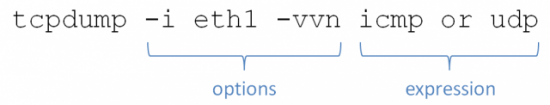
\includegraphics[width=0.5\textwidth]{figures/tcpdump_cmd.png}
    \caption{Структура на tcpdump команда.}
    \label{tcpdump_cmd_fig}
  \end{figure}

  \item \textbf{Цена} Тъй като програмата се разработва на принципа на отворения
    код, тя е изцяло безплатна и може да се използва според BSD лиценза.
  \item \textbf{Програмна поддръжка} Тъй като програмата се разработва на
    принципа на отворения код, тя няма формална поддръжка --- тя се
    базира на обществото от потребители на програмата.
  \item \textbf{Поддръжка на операционната система} Поддържа повечето
    UNIX-базирани операционни системи: Linux, Solaris, BSD, HP-UX и др.
    Microsoft Windows се поддържа през \textbf{WinDump}, която използва
    \textbf{WinPcap} --- Microsoft Windows имплементацията на \textbf{libpcap}.
\end{itemize}


\begin{figure}[h!]
  \centering
  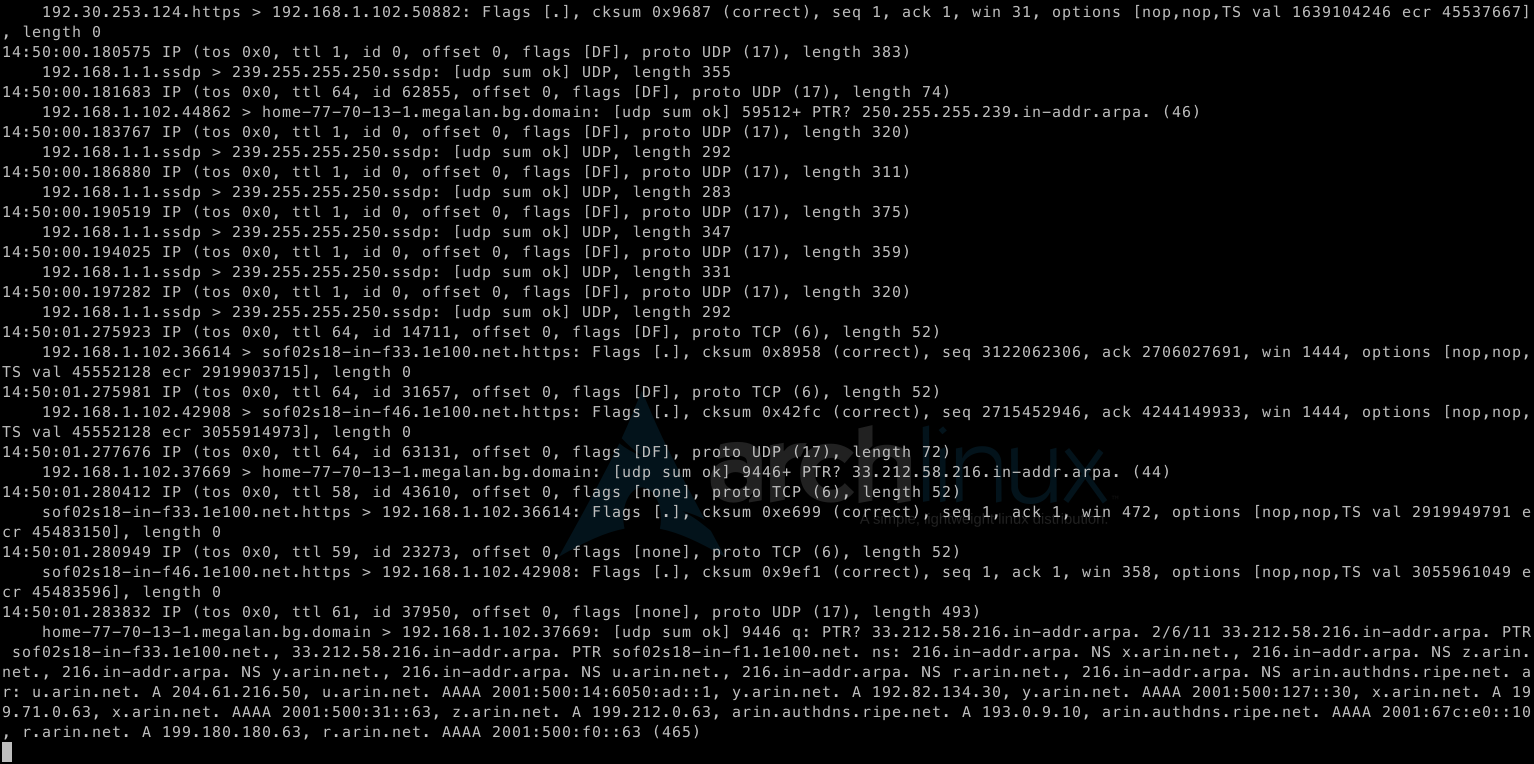
\includegraphics[width=1.0\textwidth]{figures/tcpdump.png}
  \caption{Изглед на потребителския интерфейс на tcpdump.}
  \label{tcpdump_fig}
\end{figure}

\chapter{Проектиране на структурата на мрежов анализатор}

\section{Функционални изисквания към мрежов анализатор}

\subsection{Намиране и избиране на физически интерфейси}

Преди да започне какъвто и да било анализ, мрежовия администратор трябва да
получи списък с интерфейси поддържани от мрежовата карта. Списъкът трябва да
съдържа освен имената на интерфейсите (напр. eth0), конфигурираният IP адрес,
мрежова маска с цел по-лесното ориентиране в случай на голям списък.
Анализатора трябва да предостави възможност на администратора за избор на
конкретен интерфейс, който да бъде анализиран.

\subsection{Интерпретиране на данни}

Мрежовия анализатор трябва да може да интерпретира прихваната от преносвателната
среда поредица от байтове. Тъй като типично тя е в двоичен вид, информацията за
съдържанието на пренесения PDU трябва да е в разбираем от администратора вид,
т.е представена като символен низ. Фундаментална е функционалността за
интерпретиране на най-често срещаните протоколи в TCP/IP стекът, а именно
Ethernet, IP, TCP, UDP.

\subsection{Филтриране на данни}

Прихващането на трафик директно от преносвателната среда предполага огромно
количество данни, особено в случай на голямо количество станции. Филтрирането
позволява на администратора да се абстрахира от ненужния му трафик като настрои
анализатора да приема конкретен тип трафик, напр. единствено IP трафик. В
противен случай анализирането би отнело ненужно време и ресурси.

\subsection{Отдалечен анализ}

Посредством client-server архитектура, анализатора трябва да поддържа отдалечен
анализ. Клиентът трябва да има възможност да задава команди на сървърът, а той
да ги изпълнява, делегирайки част от тях на анализатора за изпълнение.
Комуникацията между клиента и сървъра трябва да е full-duplex и в реално време с
оглед принципа на работа на мрежовия анализатор.

\subsection{Сигурност на отдалечения анализ}

С оглед на допълнителна сигурност, анализатора трябва да използва библиотека за
комуникация между сървърът и клиента поддържаща SSL, тъй като евентуалната липса
на поддръжка на криптиран трафик би довела до eavesdropping на комуникацията
между двете и следователно до анализирания трафик, достигащ до сървърa.

\subsection{Споделяне на анализа}

Анализатора трябва да има възможност за споделяне на анализа, т.е да поддържа
списък от клиенти, които едновременно да получават прихванатия трафик. 

\subsection{Сигурност на споделяне на анализа}

Анализатора трябва да поддържа метод за аутентикация, който позволява единствено
ауторизирани мрежови администратори да достъпват текущата сесия на
анализ. Така потребител (независимо злонамерен или не), достигнал случайно до
адресa на уеб сървъра, не би имал възможност да проследи целия трафик на
машината, което би било еквивалентно на огромна дупка в сигурността.

\subsection{Графичен интерфейс и визуализация}

Анализатора трябва да поддържа лесен за използване и интуитивен графичен
интерфейс. При създаване на нова сесия на анализ, мрежовия администратор трябва
да има възможност за въвеждане на парола, за избиране на физически интерфейс, за
въвеждане на филтри и стартиране на анализатора. Прозорецът на сесията трябва да
съдържа списък с прихванати пакети и кратка информация за тях, както и
компонент показващ детайлното съдържание на избран пакет, представяйки цялата му
йерархична структура с оглед моделите разгледани на стр(?).

\section{Съображения за избор на програмни средства и развойна среда}

\subsection{C++}

Езикът C\texttt{++} е език с общо предназначение, използван предимно в сферата на
системното програмиране. Създаден през 1979г. от Бьорн Строуструп, езикът е
комбинация от механизмите за абстракция на Simula и бързината и
ефективността на C. Отчитайки поддръжката на системно програмиране,
програмния код написан на C\texttt{++} лесно взаимодейства със софтуер написан
на други езици. Тази необходимост от взаимодействие е отчетена още от началия
етап на дизайна на езика и поддръжката на C, Assembler и Fortran не изисква
допълнително процесорно време или преобразуване на структурите от данни.
\cite{stroustrup_c++_2013} С оглед на факта, че libpcap е имплементирана на C и
характеристиките на C\texttt{++}, езикът е натурален избор взимайки предвид
необходимото бързодействие при работата с високоскоростни мрежови връзки.

\subsection{libpcap}

\subsection{Angular 2 и TypeScript}

\section{Проектиране на архитектура на мрежов анализатор с отдалечен достъп}

\subsection{Цялостна архитектура}

На \autoref{client_server_abstract_fig} е представен абстрактен поглед върху
цялостната архитектура на приложението. Със стрелките е означен потока от
данни между клиентите (мрежовите администратори), сървърът и анализаторът. След
като е прихванат от преносвателената среда, пакетът се обработва, подава на
сървъра и бива изпратен до всички автентикирани клиенти (broadcast).
Междувременно комуникацията между сървъра и клиентите е двупосочна (full-duplex)
--- те могат да изпращат различни команди, напр. да се автентикират към сървъра,
да проверят дали съществува сесия, да стартират сесия и т.н.

\begin{figure}[h!]
  \centering
  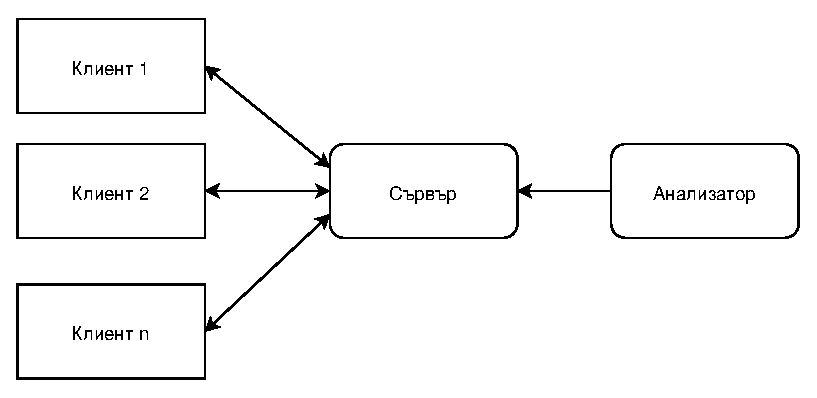
\includegraphics[scale=.7]{figures/client_server_abstract.eps}
  \caption{Абстрактен поглед върху архитектурата}
  \label{client_server_abstract_fig}
\end{figure}

\subsection{Архитектура на мрежовия анализатор}

В основата на архитектурата на мрежовия анализатор са класовете
\texttt{LayerStack} и \texttt{Layer}. Двата класа представляват частично
модифицирана имплементация на шаблона за дизайн (design pattern)
\textit{протоколен стек}. Решението, освен разделяне (decoupling) на
отговорността на слоевете, позволява динамична промяна на слоевете на стека,
напр. ако е нужно 'подпъхване' на междинен слой между два вече съществуващи с
цел криптиране, дебъгване и т.н. \texttt{LayerStack}, публичният интерфейс на
когото е описан на \autoref{layer_stack_uml_fig}, представлява двусвързан списък
от слоеве с възможност за динамично добавяне и премахване.

\begin{figure}[h!]
  \centering
  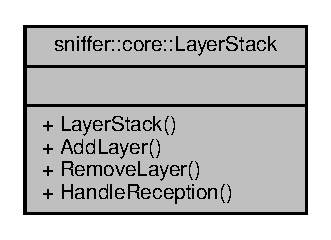
\includegraphics[scale=.9]{figures/layer_stack_uml.eps}
  \caption{UML диаграма на класа \texttt{LayerStack}}
  \label{layer_stack_uml_fig}
\end{figure}

\texttt{Layer} е базов клас за всички слоеве както е представено на
\autoref{layers_uml_fig}.  Индивидуалните слоеве се достъпват чрез указатели
от този тип. Предимството е, че конкретния тип на горния и долния слой е
неизвестен за имплементацията на даден слой.

\begin{figure}[h!]
  \centering
  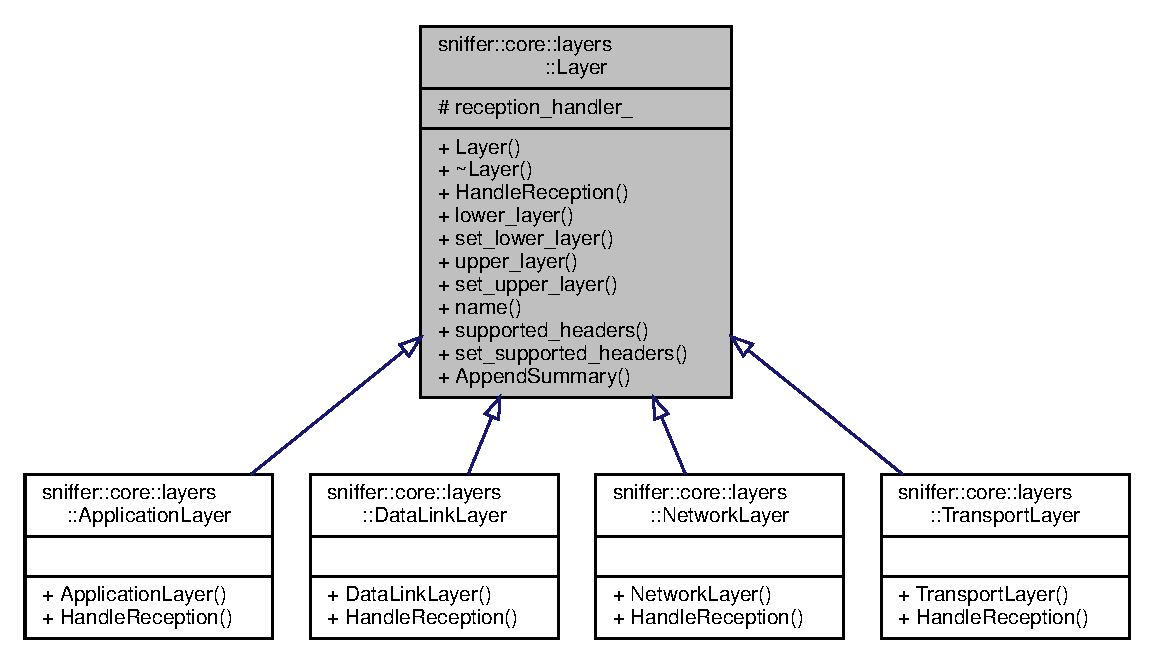
\includegraphics[scale=.7]{figures/layers_uml.eps}
  \caption{UML диаграма на класа \texttt{Layer} и наследниците му}
  \label{layers_uml_fig}
\end{figure}

Всеки обект от типа \texttt{Layer} има списък от поддържани header-и под формата
на обекти от типа \texttt{HeaderMetadata}. Например, този списък за
\texttt{TransportLayer} би съдържал обекти от типовете
\texttt{UserDatagramHeaderMetadata} и \texttt{TransmissionControlMetadata}.
На \autoref{header_metadata_uml_fig} е представен класът \textt{HeaderMetadata}.
В себе си той съдържа (?????????????).

На \autoref{sniffed_packet_uml_fig} е показан публичният интерфейс на
\texttt{SniffedPacket} класа. Той представлява частнично модифицирана
имплементация на шаблона за дизайн \textit{протоколен пакет}, още известен като
\textit{протоколен буфер} или \textit{многослоен буфер}. Взимайки предвид
описанието на (?), всеки слой добавя/премахва свой header или trailer.
Това предразполага към имплементация, в която всеки слой заделя или освобождава
нов буфер отчитайки новия размер. Изложения шаблон дава просто и ефективно
решение на този проблем.

\begin{figure}[h!]
  \centering
  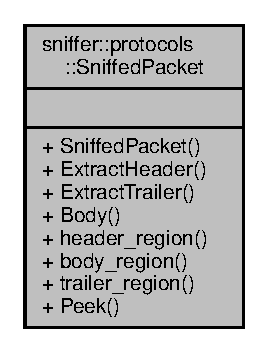
\includegraphics[scale=.7]{figures/sniffed_packet_uml.eps}
  \caption{UML диаграма на класа \texttt{SniffedPacket}}
  \label{sniffed_packet_uml_fig}
\end{figure}

Буферът стандартно се разделя на три области: header, body и trailer.
Алгоритъма на декапсулиране, представен визуално на
\autoref{sniffed_packet_regions_fig}, e следния:

\begin{enumerate}
  \item
    Полученият пакет се създава с всички байтове в body областта. В този начален
    момент, header и trailer областите имат нулева дължина.
\item
  Слой 1 изважда своите header и trailer области, двете области се "отрязват" от
  body областта. Размера на body областта се намалява.
\item
  Слой 2 също изважда своите header и trailer области, двете области отново се
  "отрязват" от body областта. Размера на body областта се намалява.
\item
  Аналогичен е процесът при трети слой, след който се получава изначалната body
  област.
\end{enumerate}

\begin{figure}[h!]
  \centering
  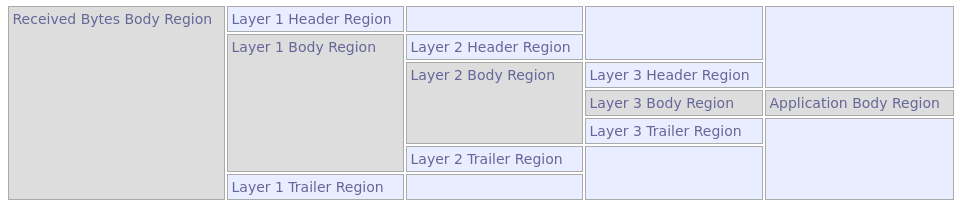
\includegraphics[width=\textwidth]{figures/sniffed_packet_regions.png}
  \caption{Диаграма на разпределение на областите при получаване на пакет}
  \label{sniffed_packet_regions_fig}
\end{figure}

Представен на \autoref{packet_sniffer_uml_fig} е абстрактния клас
\texttt{PacketSniffer} и имплементацията му \texttt{PcapPacketSniffer}.
Абстракцията е необходима с цел поддръжка на библиотеки на ниско ниво различни
от \texttt{libpcap}.  Публичният интерфейс на класа е прост --- метод, който
стартира анализатора, като в имплементацията си извиква последователно
частни виртуални методи за подготовка на физическите интерфейси, за
интерпретиране на заданените филтри и прилагането им (template method).
Всеки обект от типа \texttt{PacketSniffer} е композиран от обект от типа
\texttt{LayerStack}. С оглед имплементацията описана в (?),
\texttt{LayerStack} е де факто аналогичен, паралелен на системния протоколен
стек, но локален за мрежовия анализатор.

\begin{figure}[h!]
  \centering
  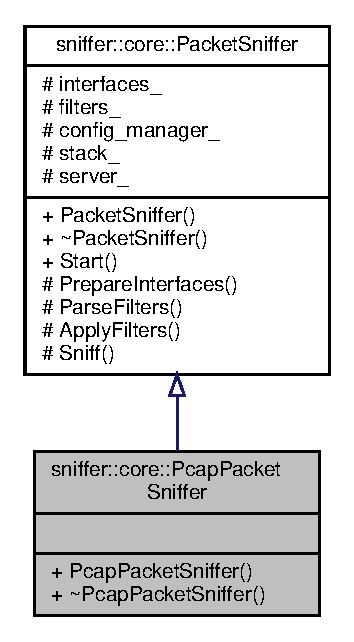
\includegraphics[scale=.7]{figures/packet_sniffer_uml.eps}
  \caption{UML диаграма на класа \texttt{PacketSniffer}}
  \label{packet_sniffer_uml_fig}
\end{figure}

\subsection{Архитектура на сървър}

\subsubsection{Ядро}

В ядрото на сървърната част на цялостната архитектура е \texttt{Server} класа.
Неговият интерфейс описва абстрактна функционалност за добавяне на нови връзки,
за множествено изпращане (broadcast), за автентикация и т.н. Абстракцията на
този клас предполага лесна подмяна на \texttt{WebSocketServer} класа, представен
на \autoref{server_websocketserver_uml_fig}, с друг тип
сървър.

\begin{figure}[h!]
  \centering
  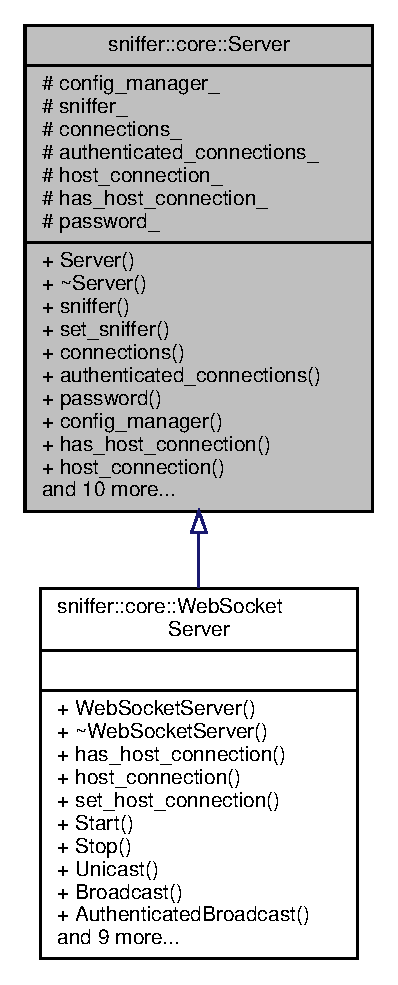
\includegraphics[scale=.7]{figures/server_websocketserver_uml.eps}
  \caption{UML диаграма на класовете \texttt{Server} и \texttt{WebSocketServer}}
  \label{server_websocketserver_uml_fig}
\end{figure}

\subsubsection{Поддръжка на команди}

\begin{figure}[h!]
  \centering
  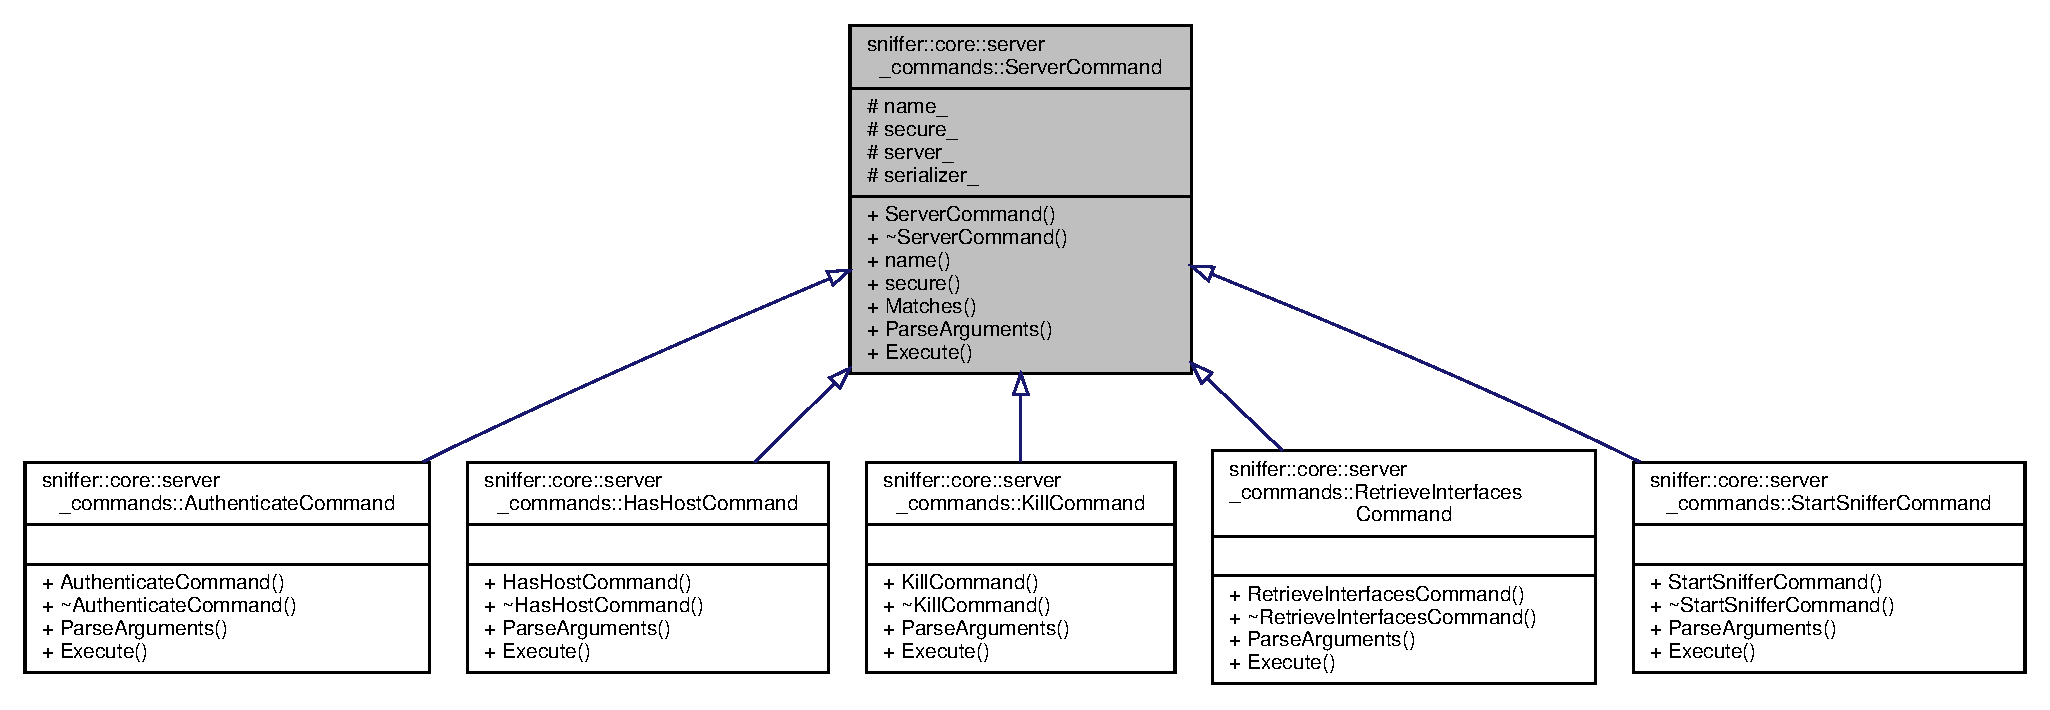
\includegraphics[scale=.5]{figures/server_command_uml.eps}
  \caption{UML диаграма на класа \texttt{ServerCommand} и наследниците му}
  \label{server_command_uml_fig}
\end{figure}

\subsection{Архитектура на клиент}

\chapter{Програмна реализация на мрежов анализатор}

\chapter{Ръководство на потребителя}

\chapter{Заключение}

\begin{appendix}
\chapter{Изходен код}
\label{app_ex1}

%\section{Appendix}
%
%For many reasons some concept may be important for the document but too long for the main text. In this kind of cases these concept can be presented with the environment \imp{appendix} in appendices, e.g., as in \autoref{app_ex1} and \autoref{app_ex2}.

%%%%%%%%%%%%%%%%%%%%%%%%%%%%%%%%%%%%%%%%%%%%%%%%%%%%%%%%%%%
%%%%%%%%%%%%%%%%%%%%%%%%%%%%%%%%%%%%%%%%%%%%%%%%%%%%%%%%%%%

%\section{Footnotes}
%
%You may want to give additional information to some points\footnote{Bla bla} in the text\footnote{Blu blup}.

%\section{Index}
%
%If the document is very long, it may be very useful for a lot of readers to have an index for searching key words and certain concepts (Crtl+F is usually very helpful in PDFs but not always the best solution). For this, the  package \imp{makeidx}, the commands \imp{makeindex} and \imp{printindex} and the compiling option \imp{make index} are needed. You may want to index different words like heterogeneous materials\index{Heterogeneous materials}, effective properties\index{Effective properties} and homogenization\index{Homogenization}.


%\begin{appendix}

\end{appendix}

%\bibliographystyle{plain}
\bibliographystyle{abbrvnat}
\bibliography{literature/library}

\listoffigures
\listoftables

\printindex

\end{document}
